%%%%%%%%%%%%%%%%%%%%%%%%%%%%%%%%%%%%%%%%%%%%%%%%%%%%%%%%%%%%%%%%%%%%%%%%%%%%%%%%
%2345678901234567890123456789012345678901234567890123456789012345678901234567890
%        1         2         3         4         5         6         7         8


\newcommand{\Bq}{\mathbf{q}}
\newcommand{\Br}{\mathbf{r}}
\newcommand{\BM}{\mathbf{M}}
\newcommand{\Bg}{\mathbf{g}}
\newcommand{\Bh}{\mathbf{h}}
\newcommand{\BJ}{\mathbf{J}}
\newcommand{\BS}{\mathbf{S}}
\newcommand{\BW}{\mathbf{W}}
\newcommand{\BP}{\mathbf{P}}
\newcommand{\BI}{\mathbf{I}}
\newcommand{\BB}{\mathbf{B}}
\newcommand{\BQ}{\mathbf{Q}}
\newcommand{\BR}{\mathbf{R}}
\newcommand{\Bzero}{\mathbf{0}}
\newcommand{\Bf}{\mathbf{f}}
\newcommand{\Btau}{\boldsymbol{\tau}}
\newcommand{\EQ}{\!\!\!=\!\!\!}
\newcommand{\EQQ}{\!\!\!\!\!\!=\!\!\!\!\!\!}
\newcommand{\Bc}{\mathbf{c}}
\newcommand{\R}{\mathbb{R}}
\newcommand{\Bv}{\mathbf{v}}
\newcommand{\BD}{\mathbf{D}}
\newcommand{\BN}{\mathbf{N}}
\newcommand{\BE}{\mathbf{E}}
\newcommand{\BC}{\mathbf{C}}
\newcommand{\BA}{\mathbf{A}}


%%%%%%%%%%%%%%%%%%%%%%%%%%%%%%%%%%%%%%%%%%%%%%%%%%%%%%%%%%%%%%%%%%%%%%%%%%%%%%%%
%% \section*{Abstract}

This chapter introduces a set of metrics to study, analyse and measure the
ability to balance for both humans and legged robots.  This set of metrics,
which we call manipulability of the center of mass, are defined based on the
concept of end-effector manipulability in the literature.  Regarding the
center of mass as an end-effector and using impulsive dynamics, the metrics
are calculated to study the ability to move and accelerate this point.  They
graphically show the instantaneous change of the center of mass velocity due
to the unit weighted norm of instantaneous changes of the joint velocities or
impulses at the joints.  The proposed metrics can be computed for humans and
general legged robots with floating base and multiple contacts with the
environment in 3D space.  This chapter also provides the results of
experiments on humans to verify the application of the metrics.  In the
experiments, the centers of mass of human subjects in different configurations
are perturbed and joint torques are computed by using inverse dynamics.  The
metrics are shown to be suitable for comparing different postures in the sense
of the total required effort for balance maintenance.

%%%%%%%%%%%%%%%%%%%%%%%%%%%%%%%%%%%%%%%%%%%%%%%%%%%%%%%%%%%%%%%%%%%%%%%%%%%%%%%%
\section{Introduction}

Humans and legged robots operate in and interact with unstructured and
unpredictable environment.  The key to their safe operation is their ability
to maintain postural stability in various body configurations.  To this end,
there has been a considerable research effort in biomechanics and neuroscience
to study and understand human postural control.  Some studies investigated the
postural control in bipedal stance or walking \cite{Horak&Nashner86,
  Mergner10, Winter95}.  Other studies focused on effects of using additional
supportive contacts to the stability \cite{Babicetal14, Maki&Mcllroy97}.

In robotics many balance criteria have been proposed over the last years in
order to help to design balancing controllers.  Among them, zero moment point
(ZMP) \cite{Vukobratovic&Borovac04, Vukobratovicetal70} or center of pressure
(CoP), foot rotation indicator (FRI) \cite{Goswami99} and zero rate of change
of angular momentum (ZRAM) \cite{Goswami&Kallem04} are the most famous and
applicable ones.  Unfortunately, most of the above mentioned criteria are not
well-defined when the robot has multiple non-planar contacts with its
environment \cite{Goswami&Kallem04}.  The other problem with these criteria is
that none of them is able to distinguish between different balanced
configurations of a robot in terms of the ability to keep the balance.  In
other words, all balanced configurations for a robot are assumed to be the
same as long as they meet the balance criteria.  Here, we tackle this problem
and introduce a set of metrics that quantitatively evaluate the ability to
balance in different postural and contact configurations.  These metrics,
which are defined for both humans and robots, can also be applicable in
comparing different configurations in the sense of balance ability.

As the center of mass (CoM) plays a key role in a balancing motion, the
ability to balance, in both humans and robots, depends on the ability to move
and accelerate the CoM.  To define a set of proper metrics, we regard the CoM
as an end-effector and employ the basic concept of end-effector manipulability
in the literature \cite{Dotyetal95} and calculate a set of metrics which are
called manipulability of the CoM.  They measure the ability to accelerate the
CoM with the constant weighted norm of joint change of velocities or impulses
at the joints.

Unlike the end-effector manipulability which is a quite developed topic
\cite{Bowling&Khatib05, Dotyetal95, Guilamoetal06, Prattichizzoetal12,
  Yoshikawa85}, there have not been many studies on CoM manipulability in the
literature.  Naksuk and Lee \cite{Naksuk&Lee06} introduced ZMP manipulability
as an extension to the ZMP balance criterion based on the concept of dynamic
manipulability of end-effectors.  Then, Cotton \emph{et al.}
\cite{Cottonetal10} were the first to introduce dynamic manipulability of the
CoM for humanoid robots.  They used the motion equation of the robot to
calculate the acceleration of the CoM due to available torque at the joints.
Recently, Gu \emph{et al.} \cite{Guetal15} proposed feasible CoM dynamic
manipulability (FCDM) for planar humanoids.  To evaluate the feasibility of
the manipulability index, they considered the ground-contact force constraints
such as friction cone and unilaterlaity of the normal force.  However, their
proposed method is not developed for floating base robots with multiple
contacts.

In this chapter, we employ a different method for calculating the
manipulability of the CoM.  In this method, we do not work out the
relationship between joint torques and acceleration of the CoM by using motion
equations.  Instead, we apply impulses at the actuated joints and then compute
the relationship between the impulses (or instantaneous changes at the joint
velocities due to the impulses) and the instantaneous change of the CoM
velocity.  This is in fact the method that is used by Featherstone
\cite{Featherstone13,Featherstone15} to study the balance ability of robots on
a single point.  This approach allows us to derive a set of configuration
based metrics (i.e. velocity independent) which are applicable to all types of
legged (floating base) robots and also humans with different contact
conditions.  Therefore, these metrics provide a tool to study balancing
motions in humans and robots and also design better and more efficient robots
in the future.

In the calculation of the CoM manipulability, we take into account the effects
of inertial parameters as well as under-actuation and kinematics constraints.
The under-actuation is due to the floating base and kinematic constraints are
due to multiple contacts with the environment, such as hands and feet for
biped robots or humans.  As a result of the manipulability analysis, we obtain
two types of ellipsoids which graphically show 1) instantaneous change of the
CoM velocity due to the weighted unit norm of impulses at the actuated joints,
and 2) instantaneous change of the CoM velocity due to the weighted unit norm
of instantaneous changes of joint velocities.  These ellipsoids, which are
calculated by using impulsive dynamics, take into account the ability to cause
the motion at the CoM.  The first type of ellipsoid shows how a certain amount
of torque at the joints can accelerate the CoM.  This can be used to study the
efficiency in the sense of required torque.  The second ellipsoid shows the
ability to move the CoM with a certain amount of movement at the joints.  This
ability can be considered as maneuverability for a human or a robot: the
higher the maneuverability (larger ellipsoid), the less movement is required
to correct the position of the CoM.

In order to investigate the applicability of the proposed metrics for human
studies, we perform experiments on human subjects.  We study the balance
recovery motions of eleven subjects in five different configurations and
compare the total amount of torque that is done by the subjects to maintain
balance at each configuration.  We apply controlled forces to the CoM of the
subjects to provide same perturbations at the CoM in all configurations.
Then, by using inverse dynamics, we compute the average total joint torques
that is applied by the subjects at each configuration.  This allows us to rank
the configurations in terms of required torque for humans to keep their
balance.  It is shown in the experimental results (section \ref{sec:Exp}) that
our proposed metric for torque efficiency predicts the same ranking for the
selected configurations.  This illustrates that the manipulability of the CoM
is a suitable tool for studying balance in humans as well as robots.


\section{Kinematic Manipulability of The CoM}
\label{sec:KinManip}

The concept of manipulability (of end-effectors) for manipulators, first
introduced by Yoshikawa \cite{Yoshikawa85a}.  He proposed that $\sqrt{\BJ_e
  \BJ_e^T}$, where $\BJ_e$ is the Jacobian of end-effector, can be used to
measure the capability of a manipulator in a specific configuration.  He also
extended this metric to dynamic manipulability by including the dynamics
equations of manipulators \cite{Yoshikawa85}.  However, Doty \textit{et. al.}
\cite{Dotyetal95} pointed out that $\sqrt{\BJ_e \BJ_e^T}$ have no physical
meaning when dealing with general robots with a combination of different joint
types (e.g. revolute and prismatic joints).  They proposed to use a weighting
matrix to solve this issue and make consistency in the units.

To extend the manipulability concept to be used for CoM of legged robots, we
need to regard the CoM as an end-effector, and also include floating-base
dynamics and kinematic constraints (due to multiple contacts with the
environment) in the equations.  Let $\Bq \in \R^n$ denote the vector of
generalized coordinates of a robot which has $6$ virtual unactuated degrees of
freedom (DoF) due to its floating base.  Assume that there are $l$ linearly
independent kinematic constraints acting on the robot.  Therefore,
%
\begin{equation}
  \BJ_c \dot{\Bq} = \Bzero \, ,
\end{equation}
%
where $\BJ_c \in \R^{l \times n}$ is the Jacobian of the constraints.  By
defining a projector $\BP = \BI - \BJ_c^{\#} \BJ_c$, we can project any
arbitrary vector $\Bv \in \R^n$ from the joint velocity space into the null
space of the constrains as
%
\begin{equation}
  \dot{\Bq} = \BP \Bv \, .
  \label{qdot=Pv}
\end{equation}
%
Note that $\BI \in \R^{n \times n}$ is an identity matrix and superscript
${}^\#$ indicates the weighted generalized inverse as introduced in
\cite{Dotyetal93}.  Since $\BJ_c$ is full row rank, $\BJ_c^\#$ is
%
\begin{equation}
  \BJ_c^\# = \BW_q^{-1}\BJ_c^T (\BJ_c \BW_q^{-1} \BJ_c^T)^{-1} \, .
  \label{Jc+}
\end{equation}
%
Also, the followings are two useful properties of $\BP$ which can be concluded
from its definition:
%
\begin{enumerate}
\item $\BP^2 = \BP$
\item $\BP^T = \BW_q \BP \BW_q^{-1}$
\end{enumerate}
%

Now, to calculate the kinematic manipulability of the CoM, we consider a unit
weighted sphere of joint velocities as
%
\begin{equation}
  \dot{\Bq}^T \BW_q \dot{\Bq} = 1 \, ,
  \label{qdotMq=1}
\end{equation}
%
where $\BW_q$ is a symmetric positive definite matrix and is used in
(\ref{qdotMq=1}) to provide consistency in units.  In the case that all joints
are revolute joints and the robot has a fixed base, one can set $\BW_q$ to
identity.  Also one physically meaningful option for this metric is the
joint-space inertia matrix which makes (\ref{qdotMq=1}) equal to the double of
the kinetic energy (the kinetic energy would be $1/2$ in this case).

By replacing (\ref{qdot=Pv}) into (\ref{qdotMq=1}), we have
%
\begin{equation}
  \Bv^T \BP^T \BW_q \BP \Bv = 1 \, .
  \label{vPMq=1}
\end{equation}
%
Let $\Bc \in \R^3$ and $\BJ \in \R^{3 \times n}$ denote the position and
Jacobian of the CoM \cite{Sugihara&Nakamura02} in the world frame,
respectively.  Then, the velocity of the CoM will be
%
\begin{equation}
  \dot{\Bc} = \BJ \dot{\Bq} = \BJ \BP \Bv = \BJ_p \Bv \, ,
  \label{velCoM}
\end{equation}
%
where $\BJ_p \in \R^{3 \times n}$ can be regarded as the Jacobian of the CoM
in the constrained space.  Here, we assume that there is no constraint on the
movement of the CoM and therefore $\BJ_p$ is full row rank.  In case that
there are any constraints on the CoM, one can define a new coordinate frame
with axes aligned with the constraints and express $\dot{\Bc}$ and $\BJ_p$ in
the new frame.  So the Jacobian in the new frame will be full row rank but it
will have a lower dimension than $\BJ_p$.

Since $\BJ_p$ is full row rank, we can write its weighted generalized inverse
as
%
\begin{equation}
  \BJ_p^\# = \BW_q^{-1} \BJ_p^T (\BJ_p \BW_q^{-1} \BJ_p^T)^{-1} \, .
  \label{Jpinv}
\end{equation}
%
So, by using the definition of weighted generalized inverses in
\cite{Dotyetal93}, we can conclude from (\ref{velCoM}) that
%
\begin{equation}
  \Bv = \BJ_p^\# \dot{\Bc} + \BN \Bv_0 \, ,
  \label{v=JPcdot}
\end{equation}
%
where $\Bv_0 \in \R^n$ is an arbitrary vector and $\BN = \BI - \BJ_p^\# \BJ_p$
is a projector to the null space of $\BJ_p$.

Now, by replacing (\ref{v=JPcdot}) into (\ref{vPMq=1}) we will have
%
\begin{eqnarray}
  \nonumber 1 & \EQ & \dot{\Bc}^T \BJ_p^\#^T \BP^T \BW_q \BP \BJ_p^\#
  \dot{\Bc} + \dot{\Bc}^T \BJ_p^\#^T \BP^T \BW_q \BP \BN \Bv_0 \\
  \nonumber & & {} + \Bv_0^T \BN^T \BP^T \BW_q \BP \BJ_p^\# \dot{\Bc} +
  \Bv_0^T \BN^T \BP^T \BW_q \BP \BN \Bv_0 \\
  & \EQ & \dot{\Bc}^T \BJ_p^\#^T \BP^T \BW_q \BP \BJ_p^\# \dot{\Bc} + \Bv_0^T
  \BN^T \BP^T \BW_q \BP \BN \Bv_0
  \label{vPv=cdot}
\end{eqnarray}
%
Note that $\BJ_p^\#^T \BP^T \BW_q \BP \BN = \BN^T \BP^T \BW_q \BP \BJ_p^\# =
\Bzero$.  This can be proved by using (\ref{Jpinv}) and also the definition of
$\BN$.  Since both terms in the right hand side of (\ref{vPv=cdot}) are
positive, we can conclude that
%
\begin{equation}
  0 \leq \dot{\Bc}^T \BJ_p^\#^T \BP^T \BW_q \BP \BJ_p^\# \dot{\Bc} \leq 1
  \, .
  \label{velellipse+}
\end{equation}
%
By using the properties of $\BP$, which are mentioned earlier in this section,
and also knowing that $\BJ_p \BP = \BJ_p$, the above equation is simplified to
%
\begin{equation}
  0 \leq \dot{\Bc}^T (\BJ \BP \BW_q^{-1} \BJ^T)^{-1} \dot{\Bc} \leq 1 \, .
  \label{velellipse}
\end{equation}
%
Equation (\ref{velellipse}) defines an ellipsoid in the velocity space at the
CoM of the robot.  The principal axes and radii of this ellipsoid are the
eigenvectors and eigenvalues of matrix $\BJ \BP \BW_q^{-1} \BJ^T$,
respectively.  The velocity ellipsoid represents the robot's kinematic ability
to move the CoM in different directions, without considering whether or not
the robot is capable of causing such motions via its actuators.  The reason is
that, this analysis is in the velocity level and therefore the motion
equations are not involved.


\section{Dynamic Manipulability of the CoM: From Impulsive Dynamics}
\label{sec:DynManip}

In this section, we use impulsive dynamics to study the manipulability of the
CoM.  Therefore, unlike section \ref{sec:KinManip}, this section provides an
impulse-based analysis that enables us to investigate the manipulability of
the CoM at the acceleration level by involving the motion equations into the
calculations.  As a result of this analysis, we define two types of ellipsoids
which we call them \textit{change-of-velocity ellipsoids} in this paper.  The
first type shows the effects of the unit weighted impulses at the joints on
the change of the CoM velocity.  The second one shows the change of the CoM
velocity due to the unit norm of instantaneous changes in joint velocities
(due to non-zero impulses at the actuated joints).  The former is called
\textit{unit joint impulse} and the latter is called \textit{unit joint
  velocity} in this paper.  As already mentioned, these ellipsoids can be used
to study energy efficiency and maneuverability, respectively.

Consider the motion equations of a floating-base robot as
%
\begin{equation}
  \BM(\Bq) \ddot{\Bq} + \Bh(\Bq,\dot{\Bq}) + \Bg(\Bq) = \BB \Btau +
  \BJ^T_c(\Bq) \, {\Bf}_c \, ,
  \label{MoEq}
\end{equation}
%
where $\BM \in \R^{n \times n}$ is the joint-space inertia matrix, $\Bh \in
\R^n$ is the vector of centripetal and Coriolis forces, $\Bg \in \R^n$ is the
vector of gravity force, $\BB \in \R^{n \times k}$ is the selection matrix for
the actuated joints, $\Btau \in \R^k$ is the vector of actuated joint torques
and ${\Bf}_c \in \R^l$ is the vector of the constraint forces.  The kinematic
constraints are either due to the kinematic loops in the mechanism or contacts
with the environment (assuming that there is no sliding or loss of contact).
The latter models the hands and feet contacts for a humanoid or a legged
robot.

According to impulsive dynamics (\S 11.7 in \cite{Featherstone08}), the
impulsive equation of motion for a general robot, concluded from (\ref{MoEq}),
is
%
\begin{equation}
  \BM \, \Delta \dot{\Bq} = \BB \Btau' + \Btau'_c \, ,
  \label{MoEqImpulse}
\end{equation}
%
where $\Btau'$ is the impulse at the actuated joints, $\Btau'_c = \BJ_c^T \,
\Bf'_c$ is the impulse due to the contact forces (via kinematic constraints),
$\Bf'_c$ is the impulse of the contact forces and $\Delta \dot{\Bq}$ is
instantaneous changes of joint velocities.

We solve (\ref{MoEqImpulse}) for $\Delta \dot{\Bq}$ and obtain
%
\begin{equation}
  \Delta \dot{\Bq} = \BM^{-1} \BB \Btau' + \BM^{-1} \BJ_c^T \Bf'_c \, .
  \label{Deltaqdot}
\end{equation}
%
It is known that $\BJ_c \, \Delta \dot{\Bq} = \Bzero$, due to the kinematic
constraints.  Hence,
%
\begin{equation}
  \BJ_c \, \Delta \dot{\Bq} = \BJ_c \BM^{-1} \BB \Btau' + \BJ_c \BM^{-1}
  \BJ_c^T \Bf'_c = \Bzero \, .
  \label{JcDeltaqdot=Eq=0}
\end{equation}
%
Since $\BJ_c$ is full row rank, $\BJ_c \BM^{-1} \BJ_c^T$ is invertible.
Therefore,
%
\begin{equation}
  \Bf'_c = -(\BJ_c \BM^{-1}\BJ_c^T)^{-1} \BJ_c \BM^{-1} \BB \Btau' \, .
  \label{Deltafc}
\end{equation}
%
By substituting (\ref{Deltafc}) into (\ref{Deltaqdot}), we obtain
%
\begin{equation}
  \Delta \dot{\Bq} = \BP_M \BM^{-1} \BB \Btau' \, ,
  \label{Deltaqdotfinal}
\end{equation}
%
where
%
\begin{equation}
  \BP_M = \BI - \BJ_{c_M}^{\#}\BJ_c \, ,
  \label{PH}
\end{equation}
%
and
%
\begin{equation}
  \BJ_{c_M}^{\#} = \BM^{-1} \BJ_c^T (\BJ_c \BM^{-1} \BJ_c^T)^{-1} \, ,
  \label{JCHpinv}
\end{equation}
%
is a generalized inverse of $\BJ_c$ with the joint-space inertia matrix as the
weighting matrix.  So,
%
\begin{equation}
  \Delta \dot{\Bc} = \BJ \, \Delta \dot{\Bq} = \BJ \BP_M \BM^{-1} \BB \Btau' =
  \BJ_\tau \Btau' \, ,
  \label{DeltacdotDeltatau}
\end{equation}
%
where
%
\begin{equation}
  \BJ_\tau = \BJ \BP_M \BM^{-1} \BB \, ,
  \label{Jtau}
\end{equation}
%
and $\Delta \dot{\Bc}$ is the instantaneous change of the CoM velocity.
Matrix $\BJ_\tau$ can be regarded as a Jacobian that maps the impulse $\Btau'$
to the step change at the CoM velocity.  In this paper, we assume that this
matrix is full row rank, implying that the CoM is not constrained and is
controllable in all directions.  In case that this assumption is not valid,
one can define a new coordinate frame with the axes aligned with the
constraints and uncontrollable directions of the CoM and express $\Delta
\dot{\Bc}$ and $\BJ_\tau$ in the new frame.  So the Jacobian in the new frame
will be full row rank in a lower dimension.


\subsection{Change-of-velocity Ellipsoid---Unit Joint Impulse}

In this subsection, we calculate the relationship between instantaneous change
of the CoM velocity and the unit weighted norm of impulse at the actuated
joints.  Since the actuated joints are not restricted to be the same type or
strength, we define a metric $\BW_\tau$ to unify the units and strengths of
$\Btau'$ in
%
\begin{equation}
  \Btau'^T \BW_\tau \Btau' = 1 \, ,
  \label{tauMtau=1}
\end{equation}
%
where $\BW_\tau$ is a weighting matrix.  According to
(\ref{DeltacdotDeltatau}), we can write
%
\begin{equation}
  \Btau' = \BJ_\tau^{\#} \, \Delta \dot{\Bc} + \BN_\tau \, \Btau'_0 \, ,
  \label{Deltatau}
\end{equation}
%
where $\BN_\tau = \BI - \BJ_\tau^{\#} \BJ_\tau$ and
%
\begin{equation}
  \BJ_\tau^{\#} = \BW_\tau^{-1} \BJ_\tau^T (\BJ_\tau \BW_\tau^{-1}
  \BJ_\tau^T)^{-1} \, .
  \label{Jtauinv}
\end{equation}
%
Thus, by replacing (\ref{Deltatau}) into (\ref{tauMtau=1}), we will have
%
\begin{eqnarray}
  \nonumber 1 & \EQ & (\BJ_\tau^\# \Delta \dot{\Bc} + \BN_\tau \Btau'_0)^T
  \BW_\tau (\BJ_\tau^\# \, \Delta \dot{\Bc} + \BN_\tau \, \Btau'_0) \\  
  \nonumber & \EQ & \Delta \dot{\Bc}^T \BJ_\tau^\#^T \BW_\tau \BJ_\tau^\# \,
  \Delta \dot{\Bc} + \Delta \dot{\Bc}^T \BJ_\tau^\#^T \BW_\tau \BN_\tau
  \Btau'_0\\
  \nonumber & & {}+ \Btau'_0^T \BN_\tau^T \BW_\tau \BJ_\tau^\# \Delta
  \dot{\Bc} + \Btau'_0^T \BN_\tau^T \BW_\tau \BN_\tau \Btau'_0\\
  & \EQ & \Delta \dot{\Bc}^T \BJ_\tau^\#^T \BW_\tau \BJ_\tau^\# \,
  \Delta \dot{\Bc} + \Btau'_0^T \BN_\tau^T \BW_\tau \BN_\tau \Btau'_0
  \label{deltatauMtaudeltatau=1}
\end{eqnarray}
%
Note that $\Delta \dot{\Bc}^T \BJ_\tau^\#^T \BW_\tau \BN_\tau \Btau'_0 =
\Btau'_0^T \BN_\tau^T \BW_\tau \BJ_\tau^\# \Delta \dot{\Bc} = 0$.  Hence,
%
\begin{equation}
  0 \leq \Delta \dot{\Bc}^T \BJ_\tau^\#^T \BW_\tau \BJ_\tau^\# \, \Delta
  \dot{\Bc} \leq 1
\end{equation}
%
and therefore
%
\begin{equation}
  0 \leq \Delta \dot{\Bc}^T (\BJ_\tau \BW_\tau^{-1} \BJ_\tau^T)^{-1} \, \Delta
  \dot{\Bc} \leq 1 \, .
  \label{torqueellipse}
\end{equation}
%
The above equation defines an ellipsoid in the acceleration space which
represents instantaneous change of the velocity of the CoM due to the unit
weighted sphere of impulses at the actuated joints.  This ellipsoid is
characterized by the eigenvectors and eigenvalues of matrix $\BJ_\tau
\BW_\tau^{-1} \BJ_\tau^T$.  According to (\ref{torqueellipse}), this ellipsoid
captures the effect of both under-actuation (due to the floating base) and
kinematic constraints (due to the contacts) in the relationship between
instantaneous change of the CoM velocity and impulses at the joints.
Therefore, it is claimed to be a proper tool to study energy efficiency in
balancing motions.  We verify this claim in the next section by performing
experiments on humans.


\subsection{Change-of-velocity Ellipsoid---Unit Joint Velocity}

Here, we calculate instantaneous change of the CoM velocity due to the unit
weighted norm of instantaneous changes of joint velocities.  First, we
consider same equation as (\ref{qdotMq=1}) for instantaneous changes of joint
velocities as
%
\begin{equation}
  \Delta \dot{\Bq}^T \BW_q \, \Delta \dot{\Bq} = 1 \, .
  \label{Deltaqdot=1}
\end{equation}
%

Before substituting (\ref{Deltaqdotfinal}) into the above equation, note that
$\BP_M \BM^{-1} \BB$ is not always full column rank, implying that it might
have a null space of \emph{internal forces}.  Internal forces are torques that
the actuators can apply that may affect the ground-reaction and contact
forces, but do not cause any motion.  Let $\BC$ denote the matrix containing
independent columns of $\BP_M \BM^{-1} \BB$.  Therefore, $\BC$ is a $n \times
rank(\BP_M \BM^{-1} \BB)$ matrix.  This matrix satisfies
%
\begin{equation}
  \Delta \dot{\Bq} = \BC \Btau_r' \, ,
  \label{Deltaqdot=Ctaur}
\end{equation}
%
where $\Btau_r'$ is a reduced vector of actuator torques having the property
that $\BC \tau_r' = \BP_M \BM^{-1} \BB \Btau'$.  Now, by replacing
(\ref{Deltaqdot=Ctaur}) into (\ref{Deltaqdot=1}) we will have
%
\begin{equation}
  \Delta \dot{\Bq}^T \BW_q \Delta \dot{\Bq} = 1 = \Btau'_r^T \BC^T \BW_q \BC
  \Btau'_r \, .
  \label{taurTC=1}
\end{equation}
%
By regarding $\BW_r = \BC^T \BW_q \BC$ as a new weighting matrix, the above
equation will be similar to (\ref{tauMtau=1}).  Given that
%
\begin{equation}
  \Delta \dot{\Bc} = \BJ \Delta \dot{\Bq} = \BJ \BC \Btau'_r \, ,
  \label{cdot=JCtaur}
\end{equation}
%
we can conclude from (\ref{torqueellipse}) that (also compare
(\ref{cdot=JCtaur}) with (\ref{DeltacdotDeltatau}))
%
\begin{equation}
  0 \leq \Delta \dot{\Bc}^T \, (\BJ \BC \BW_r^{-1} \BC^T \BJ^T)^{-1} \, \Delta
  \dot{\Bc} \leq 1 \, .
  \label{impulseellipsevel}
\end{equation}
%
The above equation is the equation of an ellipsoid which is characterized by
the eigenvectors and eigenvalues of matrix $\BJ \BC \BW_r^{-1} \BC^T \BJ^T$.
This ellipsoid shows the relationship between instantaneous change of the
velocity of the CoM with respect to the unit weighted norm of instantaneous
changes of joint velocities.  Thus, this ellipsoid represents the movement of
the CoM for a certain amount of movement at the joints.  The larger this
ellipsoid is, the less movement at the joints is required to move the CoM and
therefore the higher the ability to recover from an unbalanced configuration.
Note that, this ellipsoid includes the effect of under-actuation (due to the
floating base) as well as kinematic constraints (due to the contacts) by
involving $\BC$ instead of $\BP$ in the calculations (compare
(\ref{impulseellipsevel}) with (\ref{velellipse})).

Note that, the analysis presented in this section is applicable to planar
robots, in which case $n=k+3$, $\dot{\Bc} \in \R^2$ and the ellipsoids become
ellipses.


\section {Application to Design and Analysis}
\label{sec:application}

As previously mentioned in this paper, the dynamic manipulability of the CoM
is a metric that can be used to qualitatively analyse the physical ability of
a mechanism to accelerate its CoM.  The two proposed types of ellipsoids in
section \ref{sec:DynManip} represent the torque (energy) efficiency and
maneuverability of a robot in a certain configuration.  As can be seen in
(\ref{torqueellipse}) and (\ref{impulseellipsevel}), these ellipsoids are
dependent only on the physical properties of the robot (inertial parameters
and dimensions), kinematic constraints and its configuration and not on the
joint velocities or gravity and Coriolis forces.  In other words, these
ellipsoids are \textit{configuration dependent} and not \textit{velocity
  dependent}.  This is a fundamental difference between the proposed analysis
in this paper and those that are used in previous studies \cite{Cottonetal10,
  Guetal15, Naksuk&Lee06} which is due to employing impulsive dynamics for
deriving the ellipsoids' equations.

The \textit{Change-of-velocity ellipsoid---unit joint velocity} which is a
metric for maneuverability is a new concept that is first introduced in this
paper.  Previous CoM manipulability studies only talk about relationship
between CoM acceleration and joint torques by using full dynamics equations.
This is comparable with our proposed \textit{Change-of-velocity
  ellipsoid---unit joint torque}.  If we assume a unit weighted sphere of
joint torques at the actuated joints (i.e. $\Btau^T \BW_\tau \Btau = 1$) and
calculate the CoM acceleration (i.e. $\ddot{\Bc}$) via (\ref{MoEq}), we will
end up with an ellipsoid which its radii and orientation are the same as our
proposed ellipsoid in (\ref{torqueellipse}).  The equation of this new
(velocity dependent) ellipsoid will be
%
\begin{equation}
    0 \leq (\ddot{\Bc} - \ddot{\Bc}_v)^T \, (\BJ_\tau \BW_\tau^{-1}
    \BJ_\tau^T)^{-1} (\ddot{\Bc} - \ddot{\Bc}_v) \leq 1 \, ,
  \label{veldepellipsoid}
\end{equation}
%
where
%
\begin{equation}
  \ddot{\Bc}_v = -\BJ \BP_M \BM^{-1} (\Bh+\Bg) + \dot{\BJ} \dot{\Bq} - \BJ
  \BJ^\#_{CM} \dot{\BJ}_c \dot{\Bq} \, ,
  \label{cvddot}
\end{equation}
%
is the acceleration due to the gravity and Coriolis forces and also the joint
velocities.  Hence, physical properties of the robot and its configuration
(from $\BJ_\tau$) are the only factors that determine how much we can change
the CoM acceleration of the robot with a certain amount of joint torques.
Although, the total acceleration of the CoM is, of course, dependent on
$\ddot{\Bc}_v$, as well.  Therefore, proposed configuration based ellipsoids
in this paper capture dynamic behaviours of the system which are due to its
physical properties.  This makes them proper metrics to measure the physical
ability of a robot to accelerate its CoM and maintain its balance.

In order to use these ellipsoids for designing a new robot, one can optimize
the inertial parameters and dimensions of the robot and also its configuration
(i.e. all variables in $\BJ$, $\BC$ and $\BJ_\tau$) to maximize the size of
the ellipsoids in certain directions.  This will maximize the ability of the
robot to accelerate its CoM in those directions.  For example, maximizing the
size of the ellipsoids in the horizontal directions will maximize the ability
to accelerate the CoM in the horizontal and therefore increases the balance
ability of the robot.  For an existing robot, one can still optimize the
configuration of the robot (i.e. $\Bq$) in order to maximize the size of the
ellipsoids.


\subsection{Joint Limits}
\label{subsec:limits}

To derive ellipsoid equations in (\ref{torqueellipse}) and
(\ref{impulseellipsevel}), we did not consider any limits on the joint
movements.  Since the ellipsoids are configuration based metrics, considering
joint limits makes sense only if we analyse a robot in a configuration which
at least one of the joints is in (or very close to) its limit.  Therefore, we
define a selection matrix $\BA_j$ which selects the joints which are close to
their limits.  So,
%
\begin{equation}
  \BA_j \Delta \dot{\Bq} \leq \Bzero \, ,
  \label{AjDeltaqdot}
\end{equation}
%
which means that the joints that are selected by $\BA_j$ cannot move in one
direction.  Given the above new constraints, analytical solutions for the
ellipsoids in (\ref{torqueellipse}) and (\ref{impulseellipsevel}) are not
valid any more.  In this case, values of $\Delta \dot{\Bc}$ will form
subspaces inside those ellipsoids due to the extra constraints in
(\ref{AjDeltaqdot}).  We can find those subspaces by solving
(\ref{DeltacdotDeltatau}) and (\ref{cdot=JCtaur}), numerically.  Note that for
the first ellipsoid (\ref{AjDeltaqdot}) will be converted to
%
\begin{equation}
  \BA_j \BP_M \BM^{-1} \BB \Btau' \leq \Bzero \, ,
\end{equation}
%
and for the second one it will be
%
\begin{equation}
  \BA_j \BC \Btau'_r \leq \Bzero \, .
\end{equation}
%
The above constraints along with those in (\ref{tauMtau=1}) and
(\ref{taurTC=1}) determine admissible values of $\Delta \dot{\Bc}$ for the two
metrics.


\section{Experiments on Humans}
\label{sec:Exp}

To verify the application of the \textit{change-of-velocity---unit joint
  impulse} ellipsoid for human studies, we perform experiments on human
subjects.  As already mentioned, this ellipsoid can be used to measure torque
efficiency in balancing motions.  So, in the experiments, we perturb the CoM
of the subjects (by a cable-pulley mechanism) in different configurations and
measure the contact forces/moments with force/torque sensors (see
Fig.~\ref{experimentsetup}).  Then we calculate the average total torque that
is done by the subjects at each configuration and compare them with the
results of manipulability analysis.  These steps are described in the
following subsections.

\begin{figure}
  \centering
  \begin{tabular}{c}
    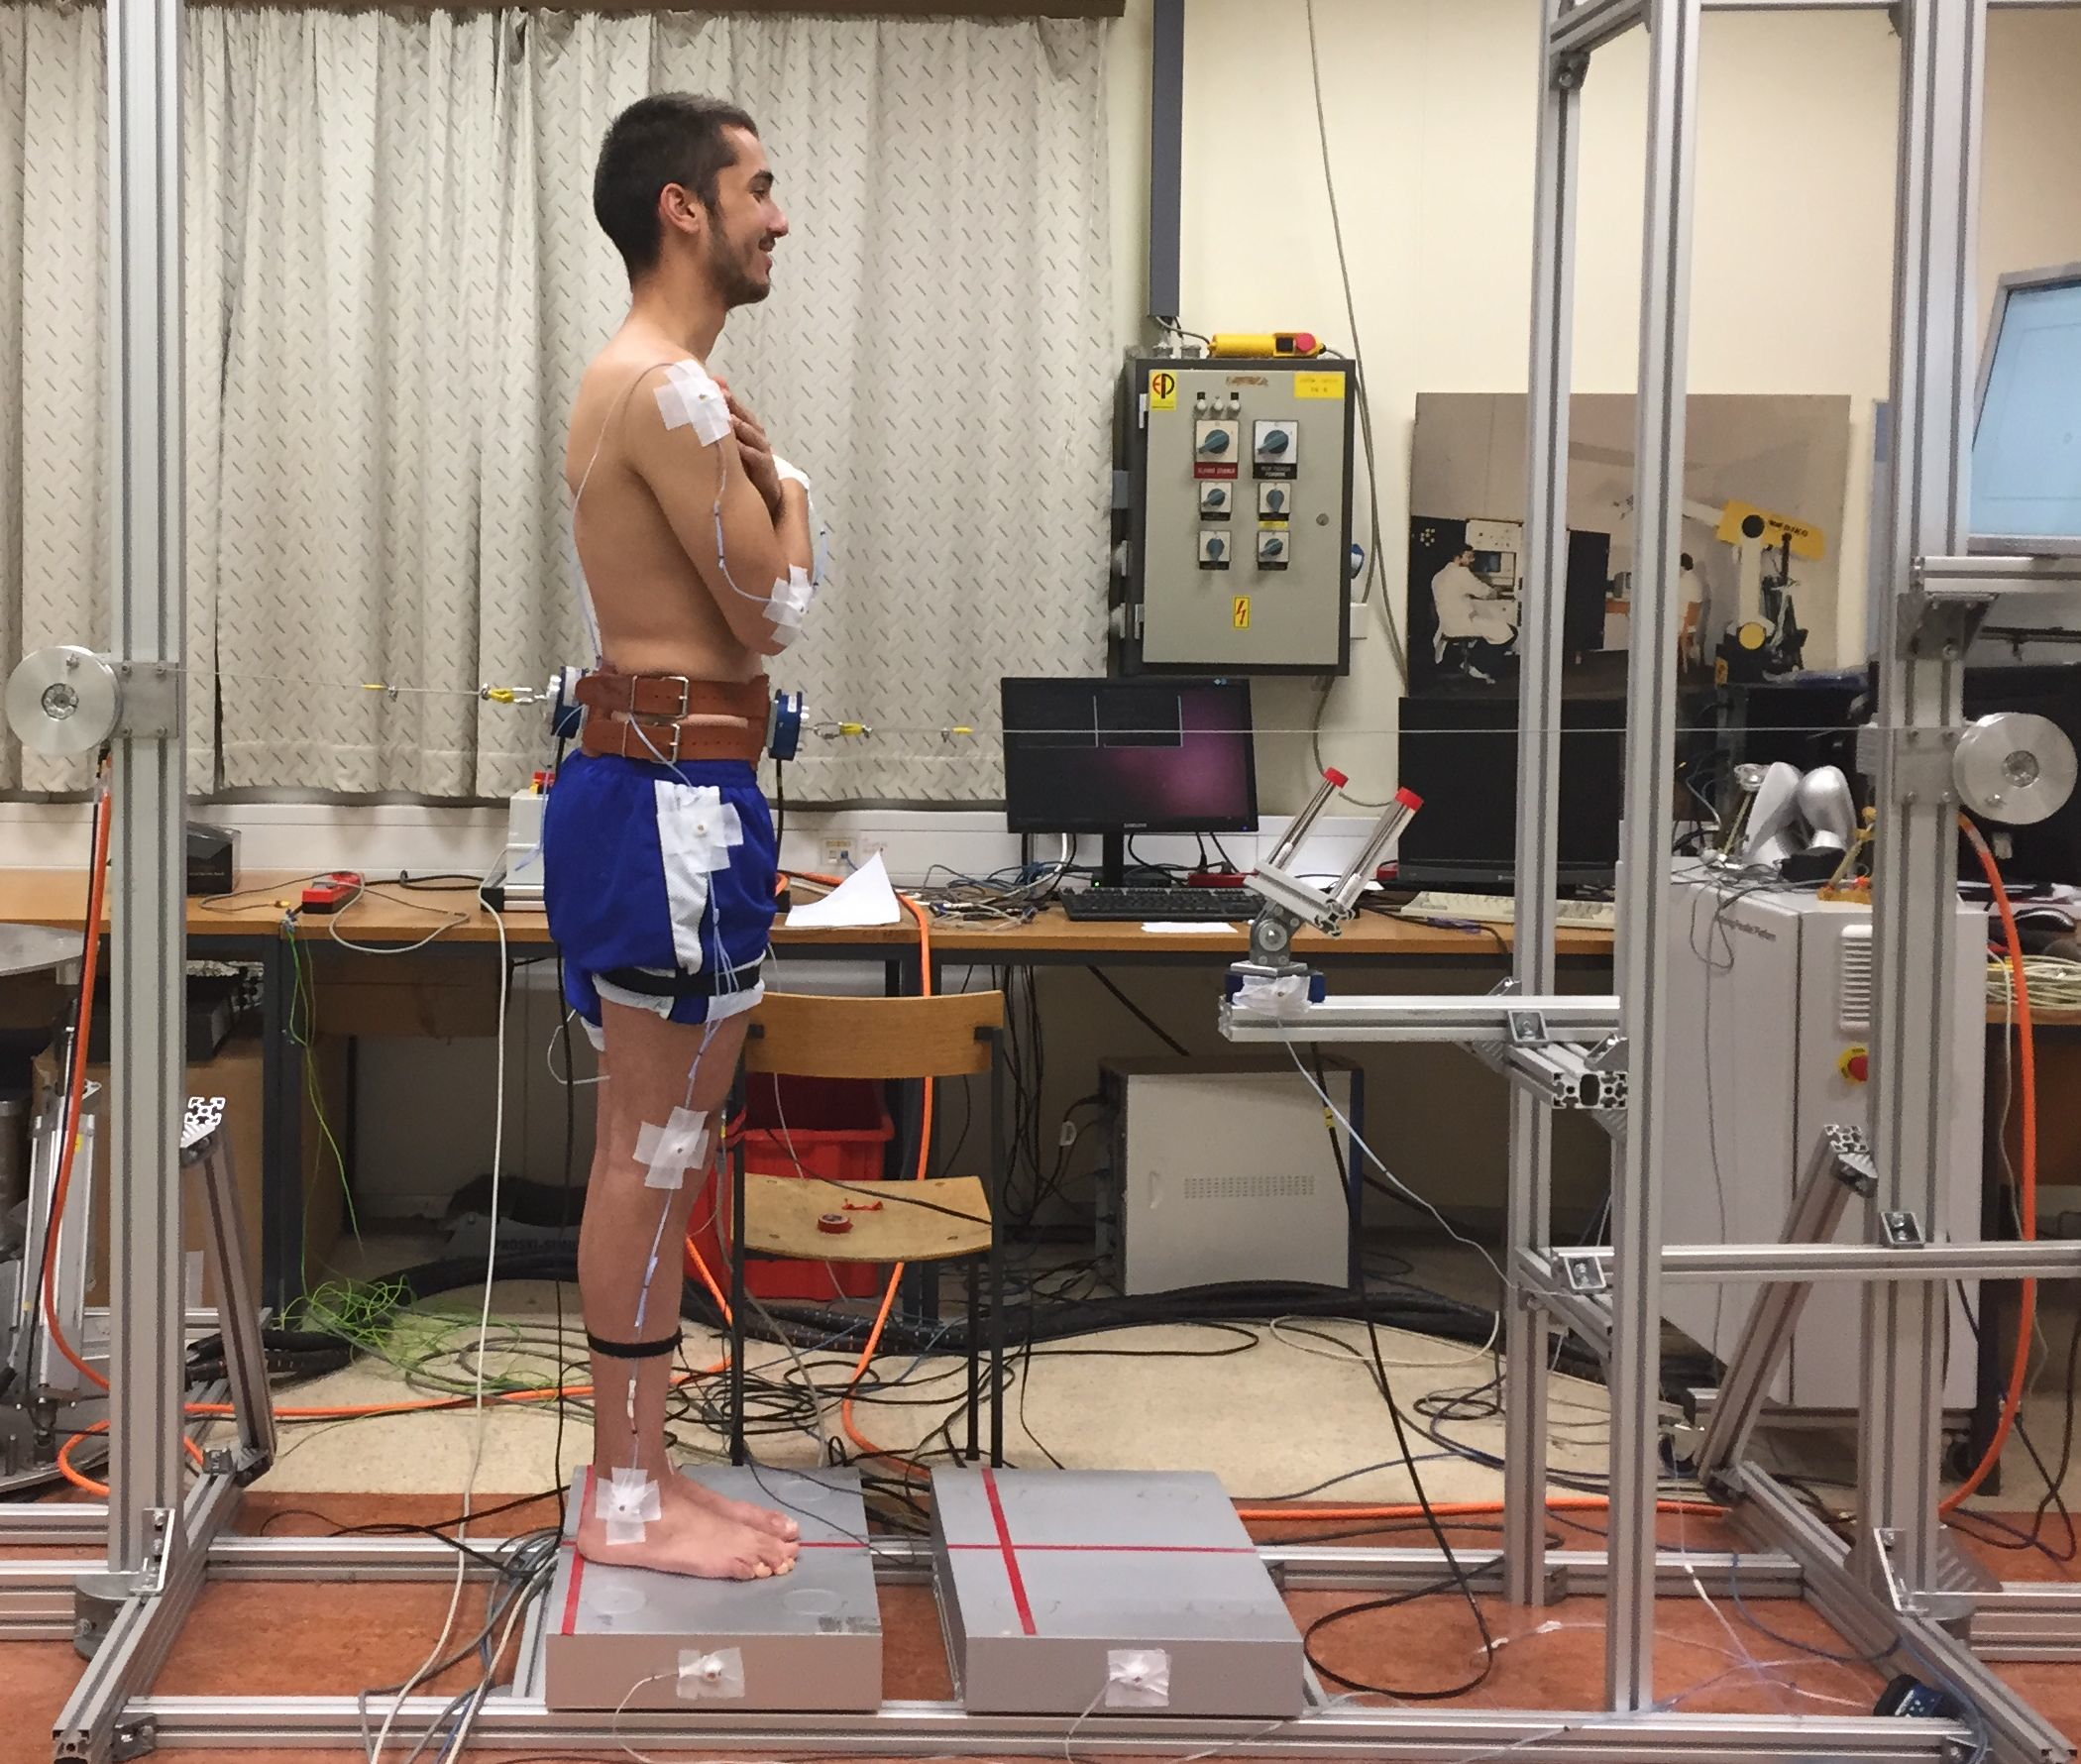
\includegraphics[width=0.75\columnwidth]{Morteza/figs/stance.jpg} \\
    (a)\\
    
  \end{tabular}
  \centering
  \begin{tabular}{cccc}
    \includegraphics[width=0.2\columnwidth]{Morteza/figs/widestance.jpg} &
    \includegraphics[width=0.2\columnwidth]{Morteza/figs/low.jpg} &
    \includegraphics[width=0.2\columnwidth]{Morteza/figs/mid.jpg} &
    \includegraphics[width=0.2\columnwidth]{Morteza/figs/high.jpg} \\
    (b) & (c) & (d) & (e)
  \end{tabular}
  \caption{Experiments setup for five different positions: (a) stance, (b)
    wide stance, (c) low handle, (d) middle handle and (d) high handle.  A
    pulley mechanism, which is connected to the subject by a belt, perturbs
    the subject's CoM. Contact forces are measured at the feet and hands.
    Motion is recorded with an optical motion capture system.}
  \label{experimentsetup}
\end{figure}


\subsection{Methods}

\subsubsection{Subjects}

Eleven healthy male subjects participated in this study.  Their average age
was $21.7$ years (SD $=2.2$ years), height = $183$ cm (SD $=4.6$ cm) and body
mass $76.8$ kg (SD $=8.1$ kg).  The subjects were informed about the course of
the study prior to their participation and were required to sign an informed
consent approved by the National Medical Ethics Committee (No. 112/06/13).


\subsubsection{Measurement Protocol}

We observed the subject’s reactions to the external perturbations in five
different poses.  In the first pose (\textit{stance}), subjects were standing
straight with their feet together and arms crossed over the torso
(Fig.~\ref{experimentsetup}.a).  In the second pose (\textit{wide stance}),
subjects were standing with their arms crossed over the torso and their left
foot $60$ cm ahead of their right foot (ankle to ankle distance).  In the
third pose (\textit{low handle}), subjects were standing as in the first pose
and holding the handle which was located in front of their bodies at the hip
height (Fig.~\ref{experimentsetup}.b).  In the fourth pose (\textit{middle
  handle}), subjects were standing as in the first pose and holding the handle
which was located in front of their bodies at the shoulder height
(Fig.~\ref{experimentsetup}.c).  In the last pose (\textit{high handle}),
subjects were standing as in the first pose and holding the handle which was
located in front of their bodies and above the head
(Fig.~\ref{experimentsetup}.d).

The subjects were perturbed by a horizontal external force produced by our
force-controlled pulling mechanism \cite{Peternel&Babic13} at the approximate
position of their CoM \cite{Gardetal04}.  The command signal was a step with
$0.5$ second width (see Fig.~\ref{perturbations}).  The actual perturbation
force was controlled by a combination of a feed-forward and a PID feedback
controller.  We selected eight linearly increasing magnitudes of perturbation
forces where the maximum was defined as 22\% of the individual subject's body
weight and the minimum was $1/8$ of the maximum force (increasing rate of
$1/8$ of the maximum).  Between each perturbation we induced a random pause.
For each pose, we repeated the series of eight perturbations ten times (80
trials per subject per pose) and observed the human reactions.  We gave the
subjects 10 minutes pause between each pose.  In case of the first pose, the
subjects had to step before the maximum perturbation was reached.  When the
subject made a step, the experimenter stopped the procedure and moved to the
next series of perturbations.  The step was not required in other poses and
the series of perturbations repeated uninterrupted.
\begin{figure}
  \centering
  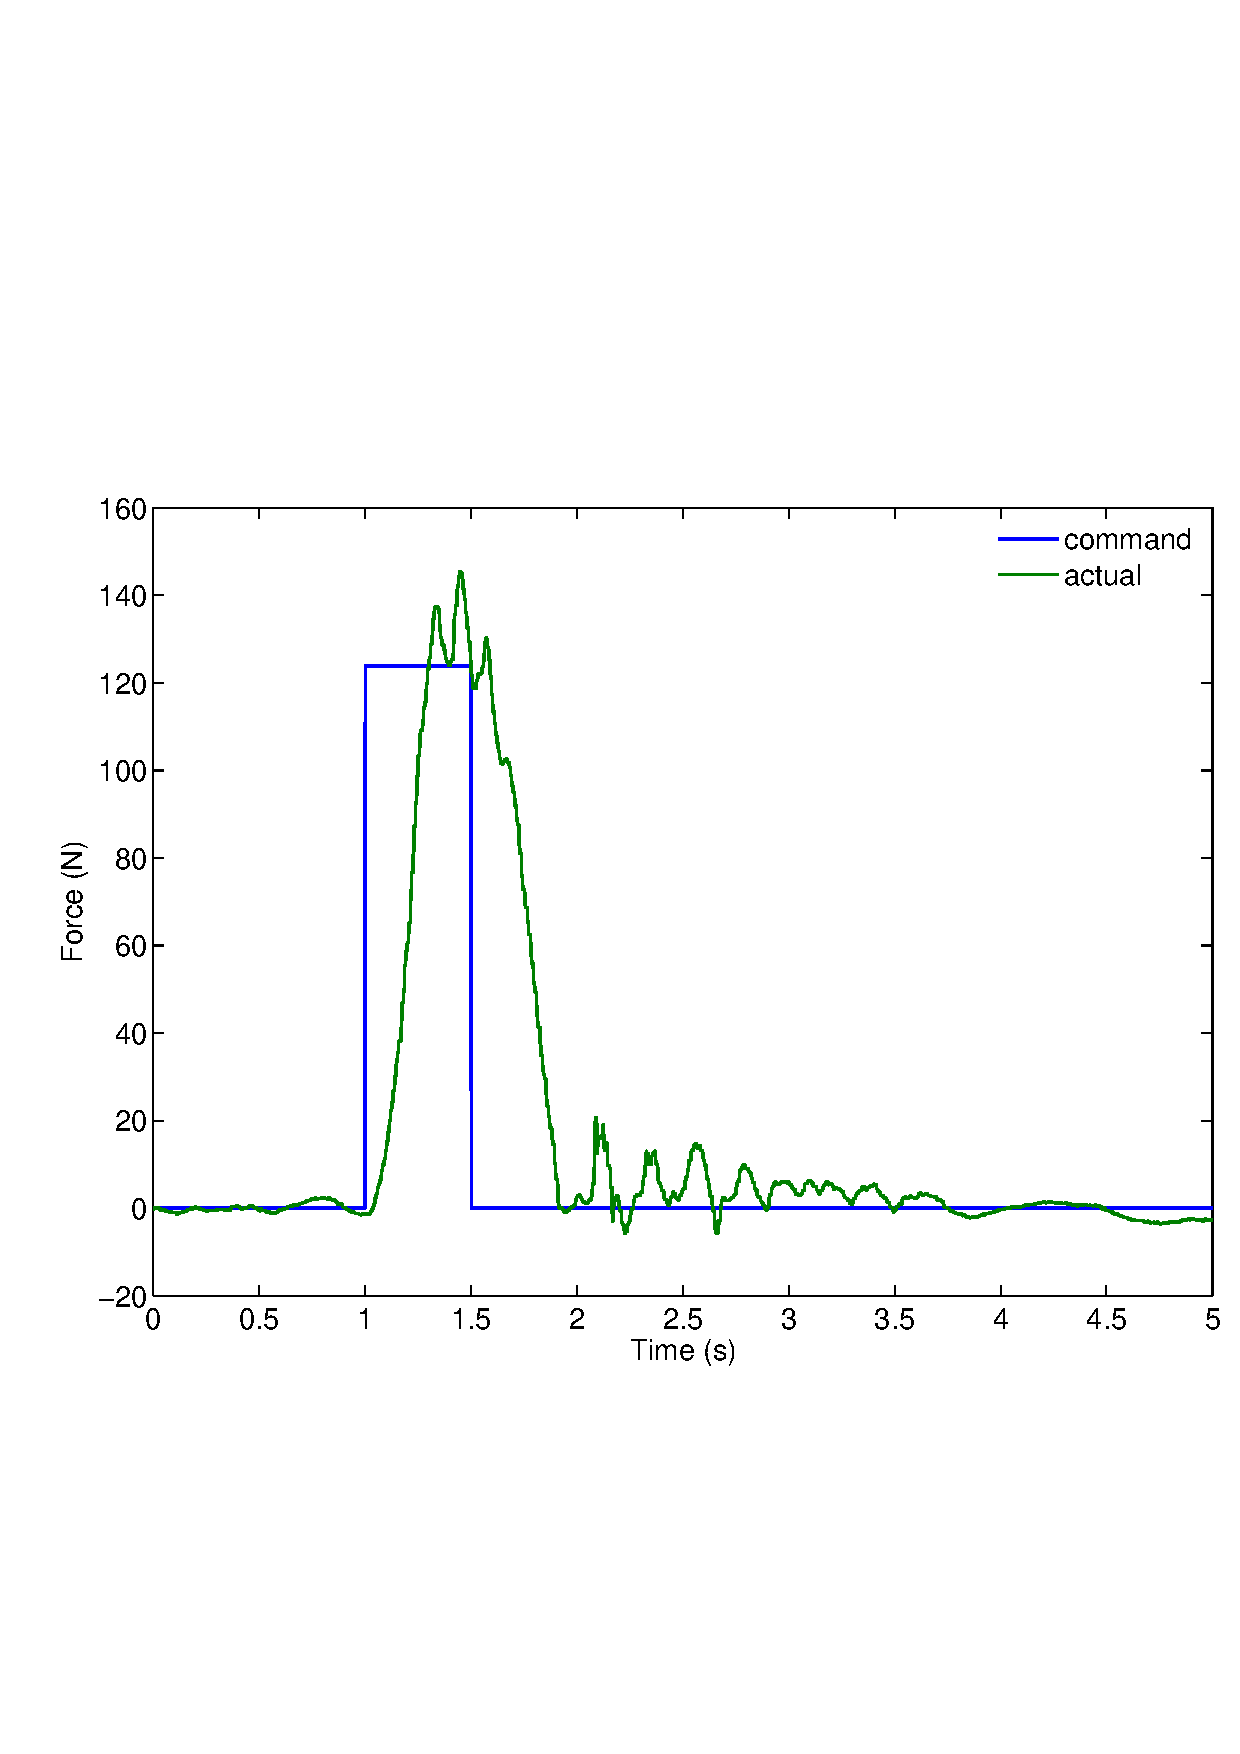
\includegraphics[scale=0.4]{Morteza/figs/perturbation.pdf}
  \caption{An example of the perturbation force applied to the CoM of the
    subjects.  This is for the subject whose body mass is $76.5$ kg.  The
    intensity of the perturbation is number $6$ meaning that the force is
    $6/8$ of the maximum for this subject.}
  \label{perturbations}
\end{figure}

Body movements were measured by a motion capture system (3D
Investigator$^{\tt\small TM}$ Motion Capture System, NDI, Waterloo, Ontario).
The optical markers were placed on the ankle, knee, hip, shoulder, elbow and
wrist.  The positions of the markers are used to calculate the joint angles.
We used two force plates (9281CA, Kistler Instrument AG, Winterthur,
Switzerland) to measure the ground reaction forces and center of pressure
position.  The handle was mounted on a 3-axis force sensor (45E15A, JR3,
Woodland, USA) to measure the force between the handle and the subject.

In order to estimate the starting time of the subjects' reactions, we measured
muscle activation in Triceps Brachii, Soleus and Tibialis Anterior by surface
electromyography (EMG).  We placed surface EMG electrodes (SX230 EMG sensor,
Biometrics Ltd, Newport, UK) on the selected muscles in accordance with SENIAM
recommendations \cite{Hermensetal99}.  We also placed a monitor in front of
the subject to provide visual feedback on the CoP position that allowed him to
move back to the initial pose after each perturbation.


\subsection{Model}

In the experiments, in order to produce movements which are planar only, we
prevented applying out-of-plane forces/moments to the subjects by providing a
pair of handles for them and perturbing them in a plane.  Therefore, we could
use planar models for both inverse dynamics and CoM manipulability
calculations.  Although, using a planar model for wide stance pose is a bit
unrealistic.  Planar humanoid models that we used for the stance, wide stance
and all three handle poses are shown in Fig.~\ref{planarhumanoids}.  These
models consist of multiple links which are connected to each other by actuated
revolute joints.  Note that lower legs are connected to the ground.  This is
because we assume that the feet of the subjects do not move during the
experiments.  To model the stance pose, we lock the DoF of the arms.  So, in
this case, the model has 3 DoF and is unconstrained.  For the wide stance, the
robot has 6 DoF and is constrained due to the kinematic loop in the legs.  For
the handle poses, the robot has five actuated DoF and it is constrained at the
hand to model the handle contact.
\begin{figure}
  \centering \includegraphics[trim = 13mm 154mm 10mm 37mm, clip,
    scale=0.85]{Morteza/figs/robotmodels}
  \caption{Schematic diagram of the planar humanoid robot model}
  \label{planarhumanoids}
\end{figure}

Since for balancing we are only interested in movements in the horizontal
direction, we calculate the maximum value of $\Delta \dot{\Bc}$ in this
direction for all five positions.  This represents the maximum achievable
change of velocity of the CoM in the horizontal direction and is a measure for
the ability to accelerate the CoM in order to correct its position in this
direction.  Due to the joint limits of the knees, instead of using
(\ref{torqueellipse}), we use the method that is described in
\ref{subsec:limits}.  Joint angles of the arms for the handle positions are
set to the average initial joint angles of the subjects that we calculate from
the marker positions.  For the low handle, the shoulder angle (angle between
torso and upper arm) is $12^\circ$ and the elbow angle (between upper and
lower arms) is $145^\circ$.  Shoulder and elbow angles are $35^\circ$ and
$77^\circ$ for the middle handle, and $96^\circ$ and $118^\circ$ for the high
handle positions, respectively.  For the wide stance position, we assume zero
angles in the knees and upright torso.  The weighting matrix that we use for
the calculations is a diagonal matrix as
%
\begin{equation}
  \BW = diag([2.33, 3.45, 4.55, 1, 1.25]) \, ,
\end{equation}
%
which is determined to include the differences in the joint's strengths
\cite{Anderson2007, Bober2002, Gandevia1998, Moraux2013}.

Calculated values for the maximum $\Delta \dot{\Bc}$ for the five positions
are mentioned in Fig.~\ref{planarhumanoids}.  As it can be seen in this
figure, the low position has the highest value (i.e. $0.17$) for the
manipulability and the stance position has the lowest one (i.e. $0.03$).
Manipulability for the middle and high positions are the same ($0.12$) and
lower than the low position.  Also wide stance manipulability (i.e. $0.09$) is
only better than the stance position.  Therefore, according to the
manipulability analysis for our models, we expect the same ranking for the
five positions in the sense of total average required torque to keep the
balance.  We will verify this hypothesis in the next subsection.


\subsection{Results}

As already mentioned, inverse dynamics are used to compute the torques that
are applied (at the joints) by the human subjects.  Joint angles are
calculated by using marker positions, and joint velocities and accelerations
are estimated by using simple time differentiation.  Lengths and inertial
parameters of the subjects are calculated via the software that is introduced
in \cite{Zlajpah&Babic14}.  Feather stone's Spatial software package
\cite{Featherstone} is used for the dynamics calculations.

To work out the average total torque for each position and each perturbation
intensity, first we calculate the joint torques from inverse dynamics for each
trial (in total $4400$ trials $= 5$ poses $\times 8$ intensities $\times 10$
reps $\times 11$ subjects).  Then we calculate the average torque over the
reps for each joint.  Note that, since maximum achievable torque of the arm
joints vary with arm configuration, we normalize shoulder and elbow torques
for the handle positions \cite{Anderson2007, Bober2002, Gandevia1998,
  Moraux2013}.  Then, we sum up the normalized joint torques to get $440$
(i.e. $5$ poses $\times 8$ intensities $\times 11$ subjects) values for the
average normalized joint torques.  The beginning time is the subjects' average
initial reaction time which is estimated by the average EMG signal.  The end
time is roughly the time that the subjects have recovered from the
perturbations.

%The same process gives us the average joint works.  The work is in fact the
%sum of $|\Btau \dot{\Bq}| \Delta t$, where $\Delta t$ is the data gathering
%frequency which is 2 milliseconds in our experiments.  We take the sum from
%$t=1.2$ s to $t=3$ s.

%% The values of the calculated normalized joint torques for the five positions
%% and different perturbation intensities are shown in
%% Fig.~\ref{jointtorquesubjects} for all subjects.  These values are marked by
%% $+$ In The graphs.  The Lines in the graphs are fitted to the values by using
%% least squares method.  Note that the graph of the first subject does not
%% include the results for high handle position.  This is due to the problem in
%% data gathering during the experiment which is solved for the next subjects.
%% \begin{figure}
%%   \centering
%%   \begin{tabular}{cc}
%%     subject 1 & subject 2 \\
%%     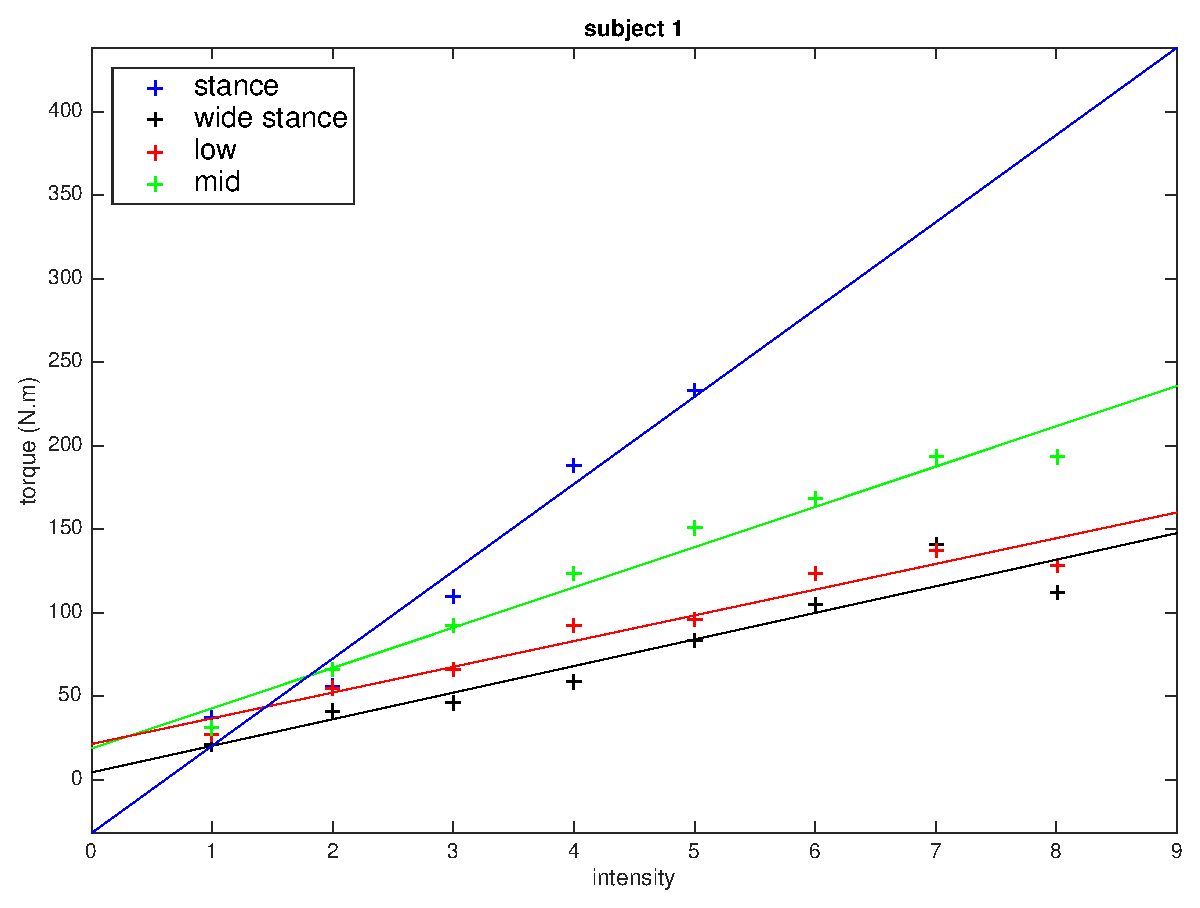
\includegraphics[width=0.46\linewidth]{Morteza/figs/subj1} &
%%     \includegraphics[width=0.46\linewidth]{Morteza/figs/subj2} \\
%%     subject 3 & subject 4 \\
%%     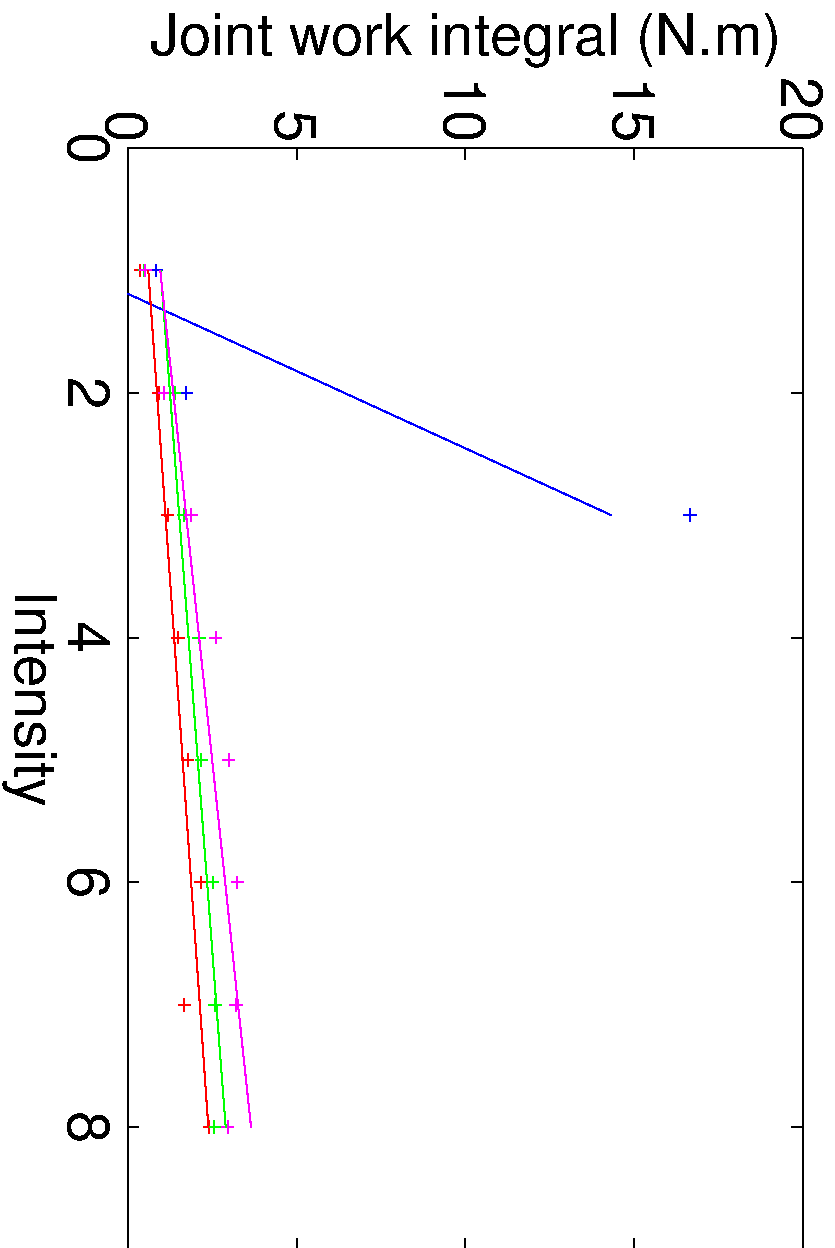
\includegraphics[width=0.46\linewidth]{Morteza/figs/subj3} &
%%     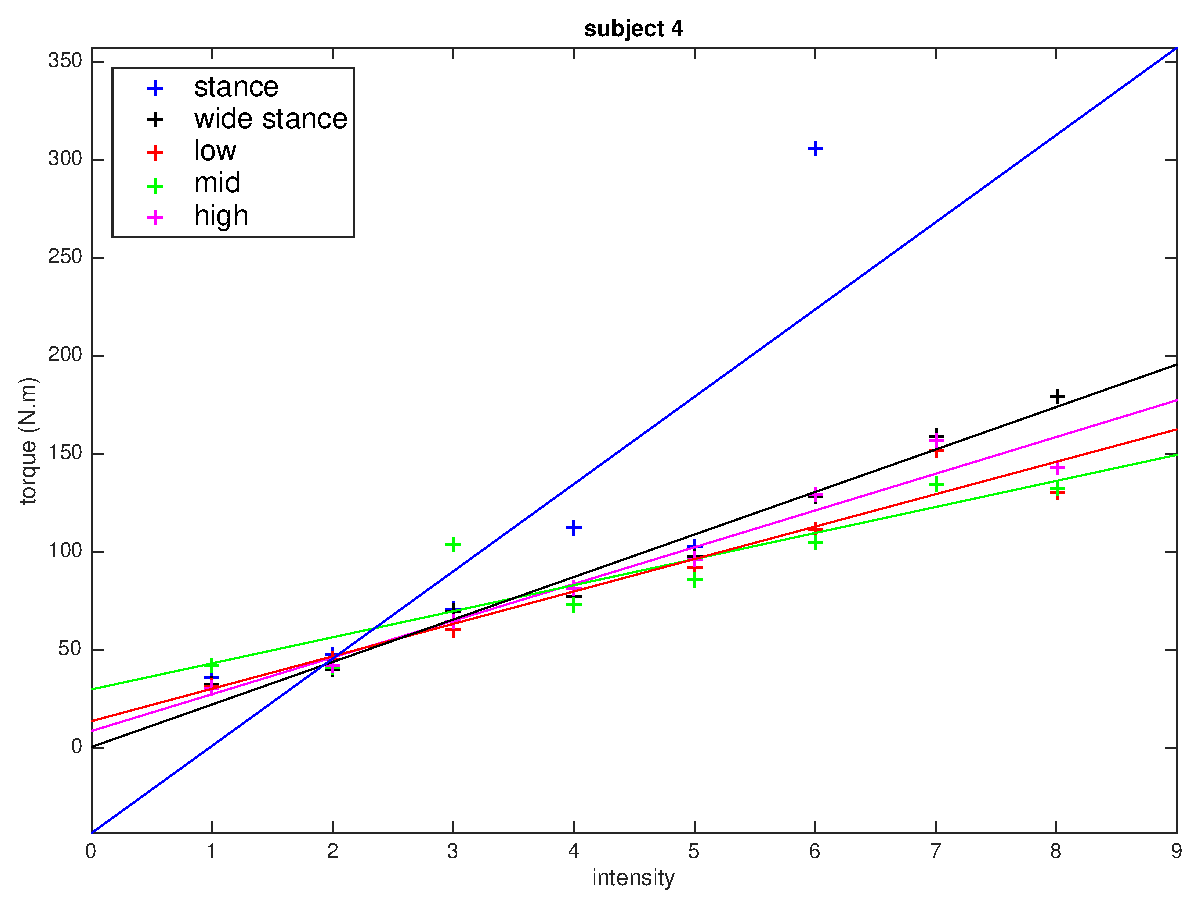
\includegraphics[width=0.46\linewidth]{Morteza/figs/subj4} \\
%%     subject 5 & subject 6 \\
%%     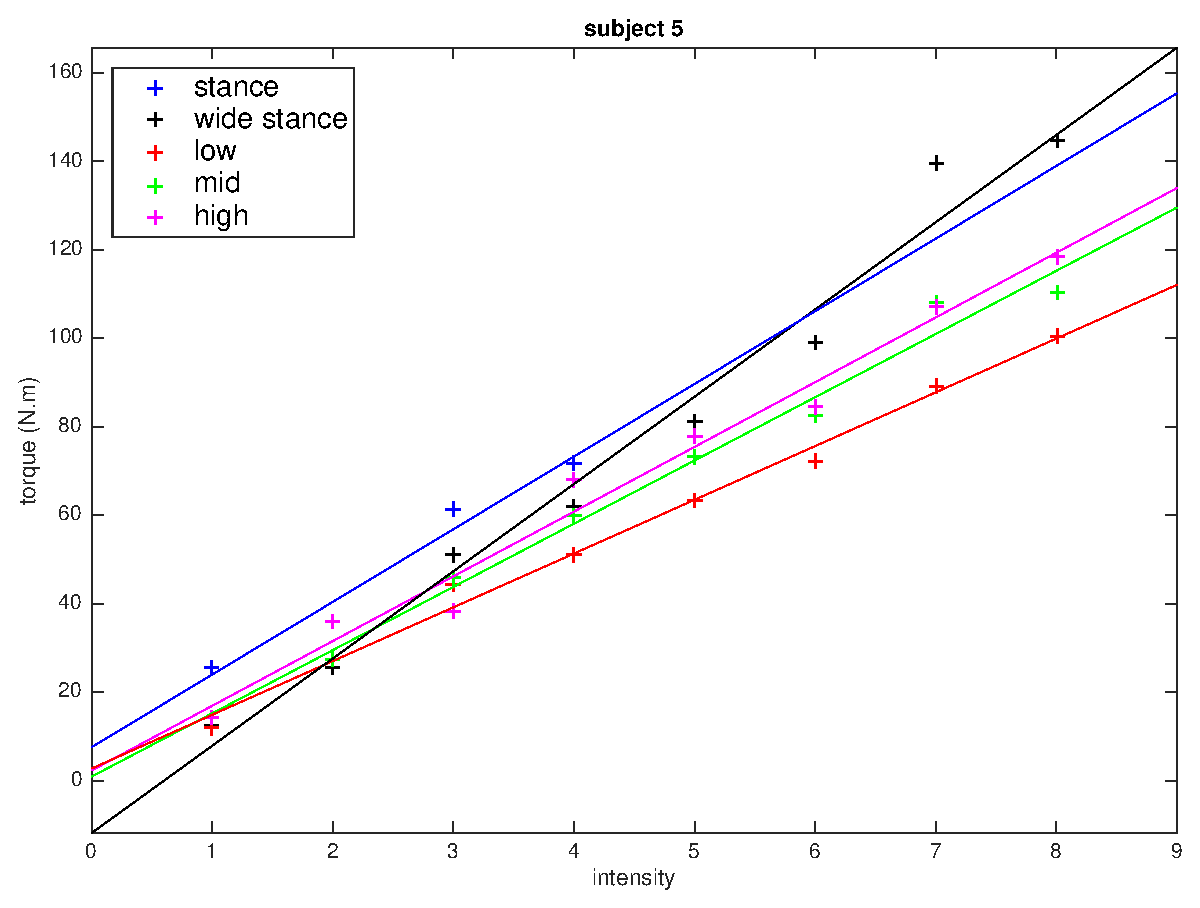
\includegraphics[width=0.46\linewidth]{Morteza/figs/subj5} &
%%     \includegraphics[width=0.46\linewidth]{Morteza/figs/subj6} \\
%%     subject 7 & subject 8 \\
%%     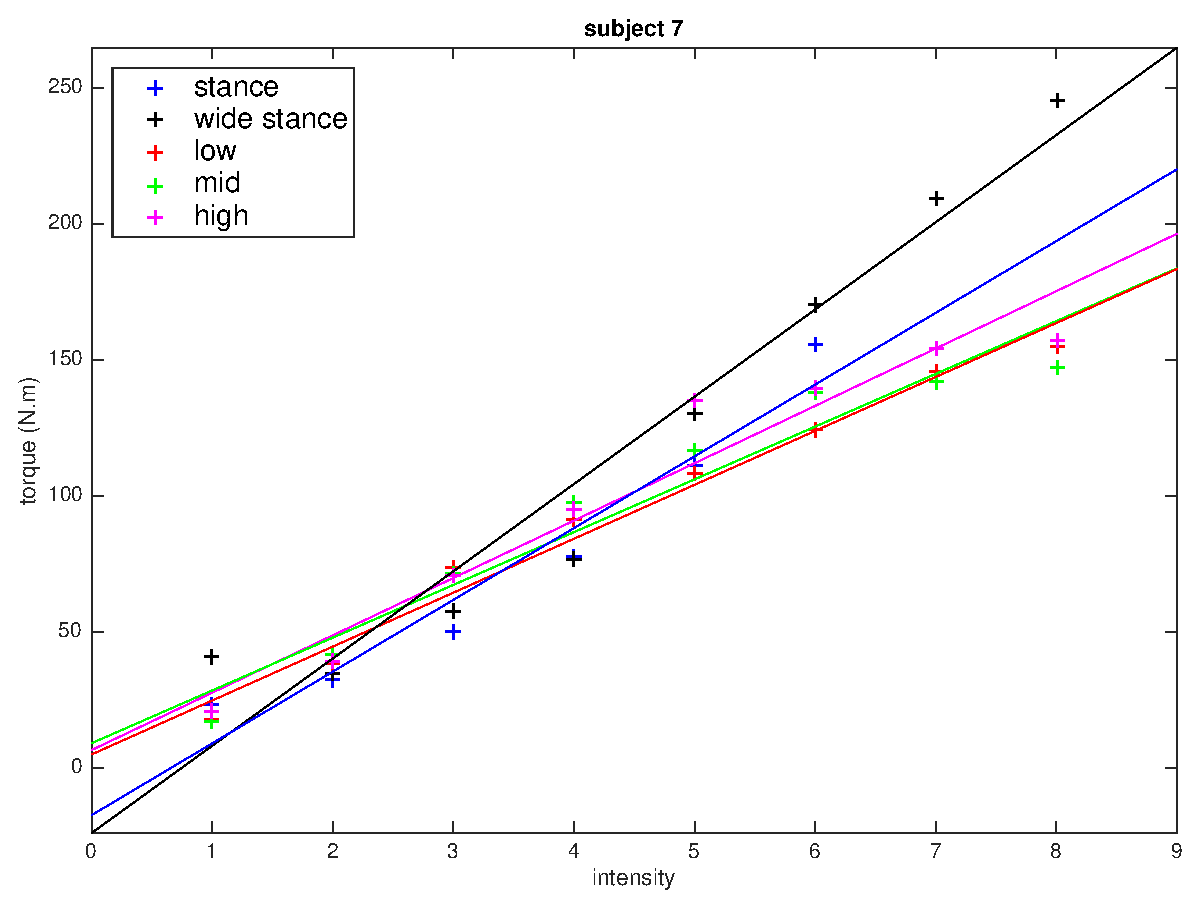
\includegraphics[width=0.46\linewidth]{Morteza/figs/subj7} &
%%     \includegraphics[width=0.46\linewidth]{Morteza/figs/subj8} \\
%%     subject 9 & subject 10 \\
%%     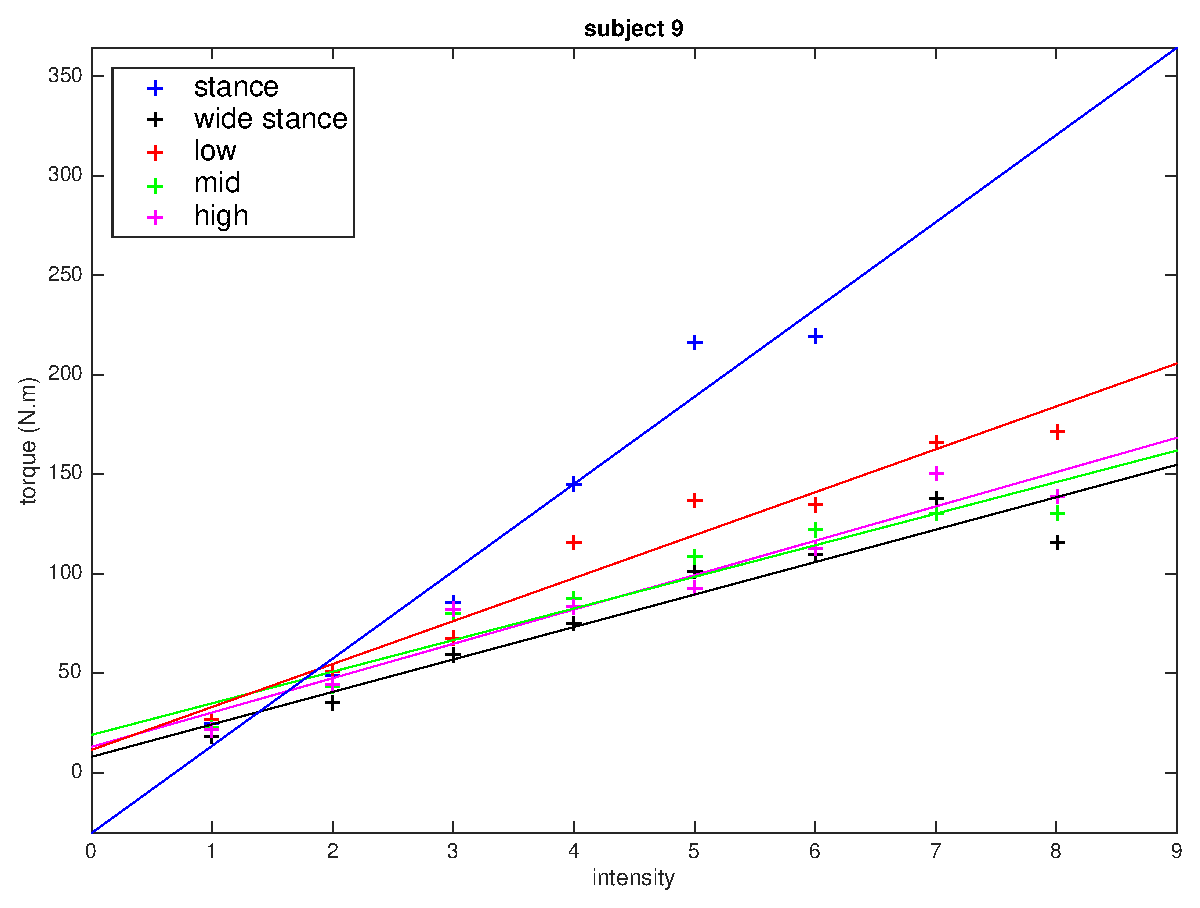
\includegraphics[width=0.46\linewidth]{Morteza/figs/subj9} &
%%     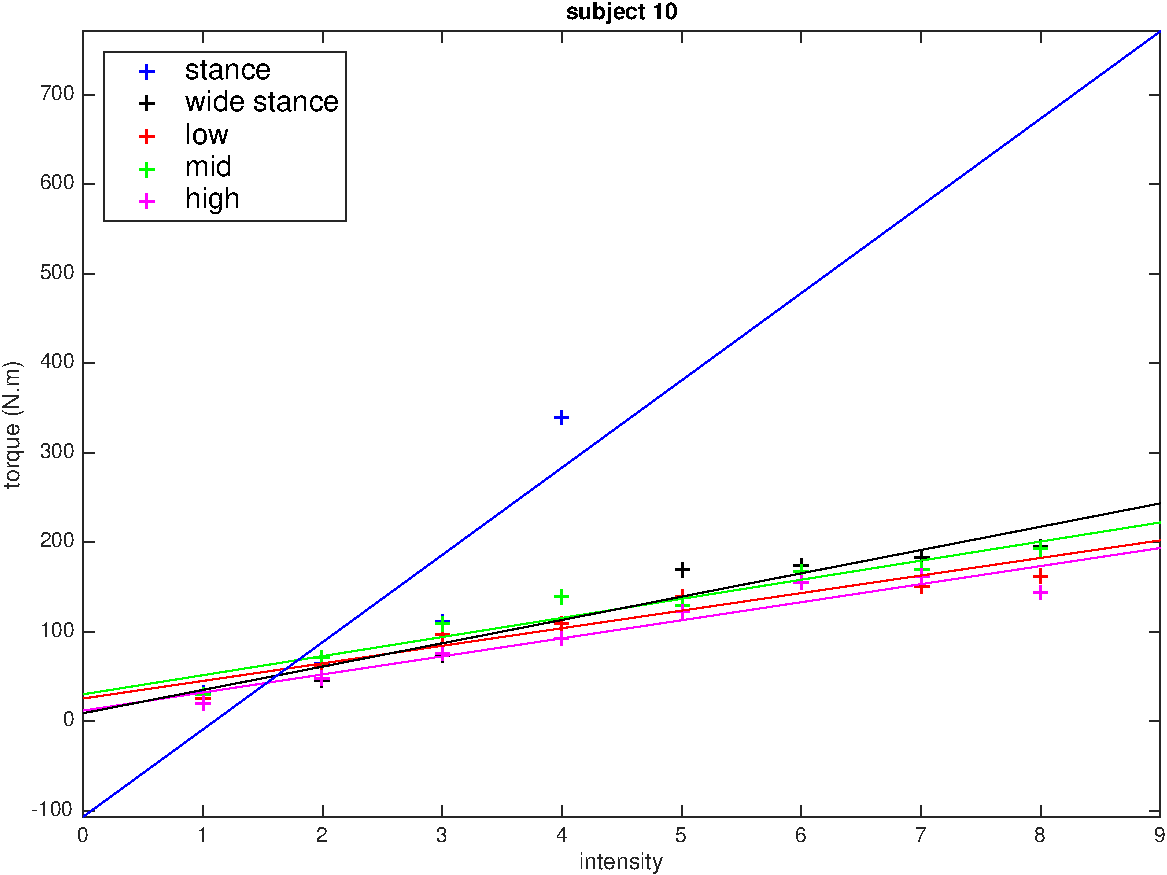
\includegraphics[width=0.46\linewidth]{Morteza/figs/subj10} \\
%%   \end{tabular}
%%   \caption{Total average normalized joint torques for the subjects at
%%     different perturbation magnitudes and different poses: stance (blue), low
%%     handle (red), middle handle (green) and high handle (magenta).}
%%   \label{jointtorquesubjects}
%% \end{figure}

The means of the normalized joint torques (per subjects) is shown in
Fig.~\ref{jointtorque}.  This figure shows the total average torque (after
removing outliers) for all subjects at each configuration and each intensity.
The lines are fitted to the values by using least squares method.  The
standard error of the means are also shown in this figure.  As can be seen in
this figure, the low handle pose has the lowest total torque and the stance
pose has the highest.  According to this graph, the ranking between the
positions is 1) low, 2) middle, 3) high, 4) wide stance and 5) stance.  This
ranking is more visible in higher intensities and it conforms with the
manipulability numbers from our analysis.  The only difference is that
manipulability analysis predicts that middle and high positions are the same
whereas experimental results show a bit difference between two (middle is
better than high).  Therefore, the experimental results agree with the
manipulability analysis in the previous subsection.  Configurations of greater
manipulability require less torque, in order to maintain balance after
perturbations of equivalent magnitudes.
\begin{figure}
  \centering \includegraphics[trim = 1mm 150mm 10mm 10mm, clip, scale =
    0.95]{Morteza/figs/errorBarPlotsSEM-norm_v2}
  \caption{Average of the total torque for the subjects at each pose and each
    perturbation intensity.  The stance position required the most torque in
    order to maintain balance.  While the low handle position required the
    least amount of torque for the same perturbation.}
  \label{jointtorque}
\end{figure}


\section{Conclusion} 
\label{sec:conclusion}

A set of metrics are introduced in this chapter to study, analyse and measure
the ability to balance for humans and robots.  These metrics, which are called
the manipulability of the center of mass, provide two types of ellipsoids
which graphically show how the CoM can be accelerated in 3D space by a certain
amount of change of motion (due to impulses) at the joint space.  These
ellipsoids can be used to measure torque efficiency and maneuverability of
humans and robots.  The proposed metrics are applicable to floating base
robots with non-breakable contacts with the environment.  Also, experiments on
human subjects are performed to investigate the applicability of the proposed
metrics for human studies.  In the experiments, the standing subjects (in five
different configurations) were perturbed by a controlled force acting on their
CoM.  Then, the selected configurations were ranked according to the average
total torque that is applied by the subjects to recover their balance at each
configuration.  It is shown that the proposed metric for torque efficiency can
successfully predict the same ranking between the configurations as the
experimental results suggested.  This agreement shows the applicability of the
metrics for human studies as well.  Therefore, manipulability of the center of
mass provides greater insight into the posture controllability of humans and
robots, in various configurations and contact conditions.


%% \section*{ACKNOWLEDGMENT}

%% The work presented in this paper is supported by the European Community
%% Framework Programme 7 through the CoDyCo project, contract no. 600716.




